%==========================================================
%
% Interactively Proving Mathematical Theorems
%
% Universidad Nacional de Colombia - Sede Manizales
%
% May 29 - June 02, 2023
%
%==========================================================
%==========================================================
\documentclass[10pt]{beamer}
\usepackage[utf8]{inputenc}
%\usepackage[brazil]{babel}
\usepackage{multicol}
\usepackage{amssymb}
\usepackage{amsmath}
\usepackage{graphicx}
\usepackage{xcolor}
\usepackage{mathtools}
\usepackage{mathrsfs}
\usepackage{fancyvrb}
\usepackage[all,2cell]{xy}
\usepackage{proof}  
\usepackage{mathpartir}
%==========================================================
%==========================================================
\usecolortheme[cmyk={0.8,0.3,0,0.6}]{structure}
    \usetheme[secheader]{Boadilla}         
    \setbeamertemplate{footline}
        {
      \leavevmode%
      \hbox{%
\begin{beamercolorbox}[wd=.333333\paperwidth,ht=2.25ex,dp=1ex,center]{author in head/foot}%
        \usebeamerfont{author in head/foot}\insertshortauthor~~%(\insertshortinstitute)
      \end{beamercolorbox}%
\begin{beamercolorbox}[wd=.333333\paperwidth,ht=2.25ex,dp=1ex,center]{title in head/foot}%
        \usebeamerfont{title in head/foot}\insertshorttitle
      \end{beamercolorbox}%
\begin{beamercolorbox}[wd=.333333\paperwidth,ht=2.25ex,dp=1ex,right]{date in head/foot}%
        \usebeamerfont{date in head/foot}\insertshortdate{}\hspace*{2em}
      \end{beamercolorbox}}%
      \vskip0pt%
    }
\usefonttheme[onlymath]{serif}
\setbeamertemplate{theorems}[numbered]    
%==========================================================
%==========================================================
%==========================================================
\newtheorem{teorema}{Teorema}[section]
\newtheorem{corolario}[teorema]{Corol\'{a}rio}
\newtheorem{lema}[teorema]{Lema}
\newtheorem{proposicao}[teorema]{Proposi\c{c}\~{a}o}
\newcommand{\demonstracao}{\noindent {\color{red}{Demonstra\c{c}\~{a}o:}} }
\newtheorem{definicao}[teorema]{Defini\c{c}\~{a}o}
%==========================================================
\newtheorem{exemplo}{Exemplo}[section]
\newtheorem{exemplos}[exemplo]{Exemplos}
\newtheorem{nota}{Nota}[section]
\newtheorem{observacao}[nota]{Observa\c{c}\~{a}o}
\newtheorem{notacao}[nota]{Nota\c{c}\~{a}o}
%==========================================================
%==========================================================
%==========================================================
\newcommand{\bck}[0]{$\backslash$}
\newcommand{\ttblue}[1]{{\color{blue!80!black}\tt#1}}
\newcommand{\ttbe}[1]{{\color{blue!80!black}\tt\emph{#1}}}
\definecolor{aquamarine}{rgb}{0.5, 1.0, 0.83}
\definecolor{darkorange}{rgb}{1.0, 0.55, 0.0}
\newcommand{\op}[1]{_{\scriptscriptstyle{#1}}}
\newcommand{\ttdo}[1]{{\color{darkorange}\tt#1}}
\newcommand{\ttaq}[1]{{\color{blue}\tt#1}}
\newcommand{\boxdarkgray}[1]{\fbox{\color{darkgray}{#1}}}
\linespread{1.3}
%==========================================================
% new commands ISR2018
%==========================================================
\newcommand{\deriv}{\bigtriangledown}
\newcommand{\cut}{\mm{(Cut)}}
\newcommand{\toesm}{\mm{(\to_e)}}
\newcommand{\toism}[1]{\mm{(\to_i){#1}}}
\newcommand{\toe}{\mm{(\to_e)}}
\newcommand{\toisa}{\mm{(\to_i)}}
\newcommand{\toi}[1]{\mm{(\to_i)\;{#1}}}
\newcommand{\landi}{\mm{(\land_i)}}
\newcommand{\lande}{\mm{(\land_e)}}
\newcommand{\landef}{\mm{(\land_{e_1})}}
\newcommand{\landes}{\mm{(\land_{e_2})}}
\newcommand{\lorif}{\mm{(\lor_{i_1})}}
\newcommand{\loris}{\mm{(\lor_{i_2})}}
\newcommand{\lori}{\mm{(\lor_i)}}
\newcommand{\lore}[2]{\mm{(\lor_e)\;{#1},{#2}}}
\newcommand{\loresa}{\mm{(\lor_e)}}
\newcommand{\loresm}[2]{\mm{(\lor_e)\;{#1},{#2}}}
\newcommand{\nege}{\mm{(\neg_e)}}
\newcommand{\negi}[1]{\mm{(\neg_i)\;{#1}}}
\newcommand{\negisa}{\mm{(\neg_i)}}
\newcommand{\nne}{\mm{(\neg\neg_e)}}
\newcommand{\nni}{\mm{(\neg\neg_i)}}
\newcommand{\nnesm}{\mm{(\neg\neg_e)}}
\newcommand{\nnism}{\mm{(\neg\neg_i)}}
\newcommand{\lem}{\rm{LEM}}
\newcommand{\pair}[2]{\mm{\langle #1, #2 \rangle}}
\newcommand{\pbc}[1]{\mm{({\rm PBC})\;{#1}}}
\newcommand{\pbcsm}[1]{(\rm{PBC}),#1}
\newcommand{\pbcsa}{(\rm{PBC})}
\newcommand{\lemcp}{(\rm{LEM})}
\newcommand{\mt}{\rm{MT}}
\newcommand{\bote}{\mm{(\bot_e)}}
\newcommand{\botesm}{\mm{(\bot_e)}}
\newcommand{\nat}{\mm{\mathbb{N}}}
\newcommand{\add}{\mm{\tt +}}
\newcommand{\lb}{\mm{\lambda}}
\newcommand{\alle}{\mm{(\forall_e)}}
\newcommand{\alli}{\mm{(\forall_i)}}
\newcommand{\exie}[1]{\mm{(\exists_e)\;{#1}}}
\newcommand{\exii}{\mm{(\exists_i)}}
\newcommand{\true}{\mm{ T}}
\newcommand{\false}{\mm{ F}}
\newcommand{\m}{{\tt m}}
\newcommand{\z}{{\tt z}}
\newcommand{\pseq}{\mbox{{\tt |---}\;}} 

\newcommand{\var}{{\sc (Var)}}
\newcommand{\app}{{\sc (App)}}
\newcommand{\absA}{{\sc (Abs)}}
\newcommand{\imp}{\to}
\newcommand{\axiom}{{\sc (axiom)}} 
\newcommand{\axiomvar}{{\sc (axiom\ var)}} 
\newcommand{\axiomtop}{{\sc (axiom\ $\top$)}} 
\newcommand{\axiombot}{{\sc (axiom\ $\bot$)}} 
\newcommand{\negation}{{\sc (negation)}} 
\newcommand{\conjunction}{{\sc (conjunction)}} 
\newcommand{\disjunction}{{\sc (disjunction)}} 
\newcommand{\implication}{{\sc (implication)}} 
\newcommand{\prop}{\rm{Prop}}
\newcommand{\tvarset}{\mathbb{V}}
\newcommand{\funset}{\mathbb{F}}
\newcommand{\predset}{\mathbb{P}}
\newcommand{\dom}{\mm{\tt D}}
\newcommand{\fv}[1]{{\tt fv}(#1)}
\newcommand{\bv}[1]{{\tt bv}(#1)}
\newcommand{\set}[1]{ \{ #1 \}}
\renewcommand{\min}[1]{ {min \{ #1 \}}}
\newcommand{\vars}[1]{\mm{{\tt var}(#1)}}
\newcommand{\subs}[2]{ \{ #1/#2 \}}
\newcommand{\fosubs}[2]{ [#1/#2]}




% Begin Commands Talk Verao 2007
\newcommand{\myboxvariable}[3]{\vspace{-3mm}$$\vbox{\hrule\hbox{\vrule\hskip#1\vbox{\vskip#1{}\hsize=#2\hsize\noindent#3\vskip#1}\hskip#1\vrule}\hrule}\vspace{-3.7mm}$$}
\newcommand\mdc{\mbox{\it gcd}}
\newcommand\LDB{\Lambda_{dB}}
\newcommand{\fd}{\to}
\newcommand{\abst}[3]{\lambda {#1}{:}{#2}.{#3}}
\newcommand\FV{{\mathcal FV}}
\newcommand\sub[3]{{#1}\{{#2}/{#3}\}}
\newcommand{\SEL}[1]{(\lambda #1)}
\newcommand{\SEA}[2]{(#1\;#2)}
\newcommand{\SEDB}[1]{{\tt \underline{#1}}}
\newcommand{\SEVr}[1]{#1}
\newcommand{\SESb}[2]{#1[#2]}
\newcommand{\SES}[3]{(#2\sigma^{#1}#3)}
\newcommand{\SEP}[3]{\varphi^{#1}_{#2}(#3)}
\newcommand{\SEDummy}{\diammond}
\newcommand{\SESp}[4]{[\![#1,#2,#3,#4]\!]}
\newcommand{\SEId}{id}
\newcommand{\SEUp}{\uparrow}
\newcommand{\SEPt}[2]{(#1\cdot #2)}
\newcommand{\SECp}[2]{(#1\circ#2)}
\newcommand{\SECon}[2]{#1::#2}
\newcommand{\SECk}[4]{\{\!\{#1,#2,#3,#4\}\!\}}
\newcommand{\SENil}{nil}
\newcommand{\SEPaar}[2]{(#1,#2)}
\newcommand{\SEAr}[1]{@#1}
\newcommand{\SELG}[4]{\langle\!\langle#1,#2,#3,#4\rangle\!
angle}


\newcommand{\rTo}{\longrightarrow}

\newcommand{\abs}[2]{\lambda_{#1}.{#2}}
\newcommand{\absG}[2]{\mbox{\color{\FigGcol}$\lambda_{#1}.{#2}$}}
\newcommand{\absR}[2]{\mbox{\color{\FigRcol}$\lambda_{#1}.{#2}$}}
\newcommand{\absB}[2]{\mbox{\color{\FigBcol}$\lambda_{#1}.{#2}$}}
\newcommand{\tyabs}[2]{\lambda_{#1}.{#2}}
\newcommand{\absb}[1]{\lambda.{#1}}
\newcommand{\absbG}[1]{\mbox{\color{\FigGcol}$\lambda.{#1}$}}
\newcommand{\absbR}[1]{\mbox{\color{\FigRcol}$\lambda.{#1}$}}
\newcommand{\absbB}[1]{\mbox{\color{\FigBcol}$\lambda.{#1}$}}
\newcommand{\absdb}[1]{\lambda {#1}}
\newcommand{\apl}[2]{({#1}\;\;{#2})}
\newcommand{\myigls}{=_{\lambda s_e}^?}
\newcommand{\igls}{=_{\lambda\sigma}^?}
\newcommand{\tvar}{{\it {\cal T}var}}
\newcommand\Sub[2]{{#1}[{#2}]}
\newcommand\Id{id}
\newcommand\Comp[2]{{#1} \circ {#2}}
\newcommand\Sh{\uparrow}
\newcommand{\substit}{{\it Subst}}
\newcommand{\vvar}{{\it var}}
\newcommand{\fvar}{{\it {\cal F}var}}
\newcommand{\beigls}{=_{\beta\eta}^?}
\newcommand \si {\,\sigma^i}
\newcommand \fik {\varphi^i_k}
\newcommand{\AND}{\ {\wedge}\ }
\newcommand{\OR}{\ {\vee}\ }
\newcommand{\IMPLIES}{\ {\Rightarrow}\ }
\newcommand{\NOT}{\neg}

%==========================================================
\title
[Mechanizing Mathematics]
{\vspace{-5mm}
%\includegraphics[scale=.35]{Marca_UFG.png}
\\%[8mm]
%{\scriptsize\bf  Universidad Nacional de Colombia - Sede Manizales}\\
{\bf\Large Mechanizing Mathematics}\\
{\large Case of Study: The infinity of prime numbers by F\"urstenberg argument} \vspace{-.1cm}}


\author[M. Ayala-Rinc\'on (UnB) \& T. A. de Lima (UFG)]
{Universidad Nacional de Colombia - Sede Manizales \\
Facultad de Ciencias Exactas y Naturales\\[6mm]
\textbf{Thaynara Arielly de Lima
  (IME)}   
\includegraphics[scale=.18]{ufg.png}\\
\textbf{Mauricio Ayala-Rinc\'on (CIC-MAT)} 
\includegraphics[scale=.03]{unb.jpg}
\vspace{-.8cm}}

\date[Universidad Nacional de Colombia - Sede Manizales]{{\scriptsize\it Funded by the Brazilian agencies CNPq, grants Universal 409003/21-2; \\ FAPDF, grant DE 00193-00001175/2021-11 and \\ FAPEG, grant 202310267000223.}
\\ May 29 - June 02 ,
  2023}  





%==========================================================
%==========================================================
\begin{document}
%==========================================================
%==========================================================
\begin{frame}
\maketitle
\end{frame}
%==========================================================
%==========================================================
\begin{frame}
\frametitle{Talk's Plan}
%----------------------------------------
\begin{columns}
\begin{column}{10cm}
%----------------------------------------
\tableofcontents
%----------------------------------------
\end{column}
\end{columns}
%----------------------------------------
\end{frame}
%==========================================================
%==========================================================

%==========================================================
%==========================================================




\section{ Infinity of Primes - Topological Argument}


\begin{frame}
\frametitle{Infinity of Primes: \\ F\"{u}rstenberg Topological Argument \cite{Furstenberg1955}, \cite{theBook2018}} 
   \begin{center}
     Our main goal in this mini-course is to formalize the Infinity of Primes following the F\"{u}rstenberg argumentation. \\
\vspace{1cm}
     Let's see the analytical proof of such fact. 
     \begin{center}
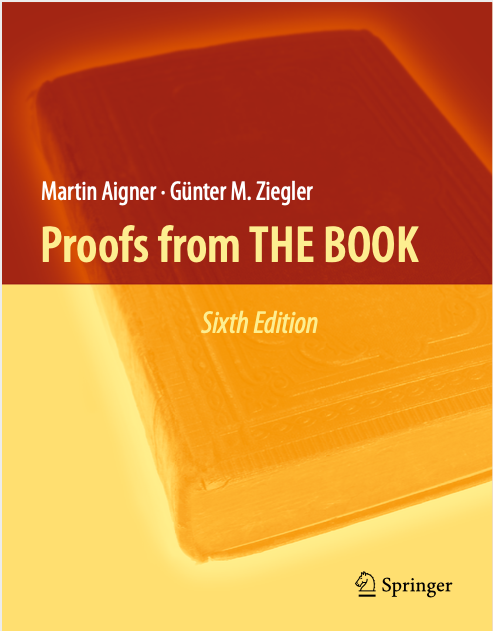
\includegraphics[scale=.15]{capa_from_the_book.png}
\end{center}
     \end{center}
 \end{frame}  


\begin{frame}
  \frametitle{Infinity of Primes: \\ F\"{u}rstenberg Topological Argument} 

  \begin{block}{Topology}

    A topology over a set $X$ is a collection
    $\tau$ of subsets of $X$ satisfying the following properties:
    \begin{itemize}
    \item[i)] $\emptyset$ and $X$ belong to $\tau$;
    \item[ii)] The union of elements of any sub-collection of $\tau$ belongs to $\tau$;
     \item[iii)] The intersection of elements of a finite sub-collection of $\tau$ belongs to $\tau$.
    \end{itemize}
\begin{itemize}
    \item A set $X$ equipped with a topology $\tau$ is called a
      \textbf{topological space}.
      \item A subset $U$ of a topological space $X$, that belongs to the collection $\tau$, is called
        an \textbf{open set of $X$}.
\end{itemize}
    
    \end{block}
   

 \end{frame} 

 % % ----------------------------------------


\begin{frame}
  \frametitle{F\"{u}rstenberg Topological Argument} 

 
    
  \begin{exampleblock}{Example}
    
Consider the sets $X = \mathbb{Z}$ and $N_{a,b} = \{ a+n \cdot b; n \in \mathbb{Z}\}$, $a, b \in
\mathbb{Z}$, where $b>0$.
A set $O \subseteq \mathbb{Z}$ is called open if and only if $O = \emptyset$ or for every $a \in O$,
there is an integer $b>0$ such that $N_{a,b} \subseteq O$.
\vspace{-7mm}
\begin{center}
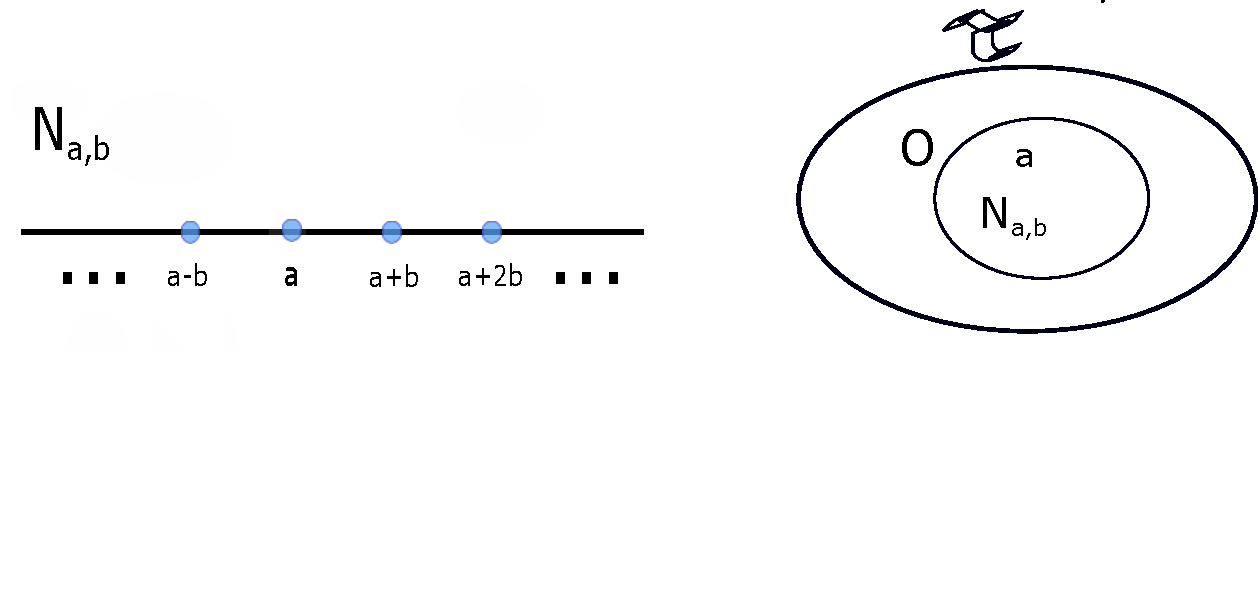
\includegraphics[scale=.3]{topology.pdf}
\end{center}
\vspace{-5mm}
\textbf{The collection $\tau$, induced by the open sets of type $O$, is a topology over $\mathbb{Z}$:}
\begin{itemize}
\item[i)] $\emptyset$ and $\mathbb{Z}$ belong to   $\tau$;
 \item[ii)] By the definition of elements of $\tau$, the
 arbitrary union of subsets of $\tau$ belongs to $\tau$;
  \item[iii)] If $O_1$ and $O_2$ belong to $\tau$ then $O_1 \cap
    O_2$ belongs to $\tau$.
    \begin{itemize}
      \item In fact, consider $a \in O_1\cap O_2$. There are $b_1$ and $b_2$ such that
      $N_{a,b_1} \subseteq O_1$ e $N_{a,b_2} \subseteq O_2$. Logo,
      $N_{a,b_1\cdot b_2} \subseteq O_1 \cap O_2$. 
      \end{itemize}
        \end{itemize} 
      \end{exampleblock}

 \end{frame} 

 % % ----------------------------------------
 \begin{frame}
   \frametitle{F\"{u}rstenberg Topological Argument}
   \begin{exampleblock}
     
   \begin{itemize}
   \item \textbf{Statement 1:} Any nonempty open set is infinite. 
     \begin{itemize}
         \item Proof: if $O \neq \empty$ then $N_{a,b} \subset O$, for some $a \in O$ and $b >0$.
       \end{itemize}
    \item \textbf{Statement 2:} For any
      $a \in \mathbb{Z}$ and $b >0$, $N_{a,b}$ is an open set. 
      \end{itemize}
    \end{exampleblock}
\pause
\begin{block}{Closed sets}

A subset $A$ of a topological space $X$ is called a closed set if and only if its complement $A^c$ is 
an open set in $X$. 
\end{block}

\begin{exampleblock}
  
  \begin{itemize}
    \item \textbf{Statement 3:}  For any
      $a \in \mathbb{Z}$ and $b >0$, $N_{a,b}$ is closed.
    \end{itemize}
    $$N_{a,b}  = \mathbb{Z} \setminus \displaystyle{\bigcup_{i=1}^{b-1}N_{a+i,b}}$$
    \vspace{-7mm}
   \begin{center}
 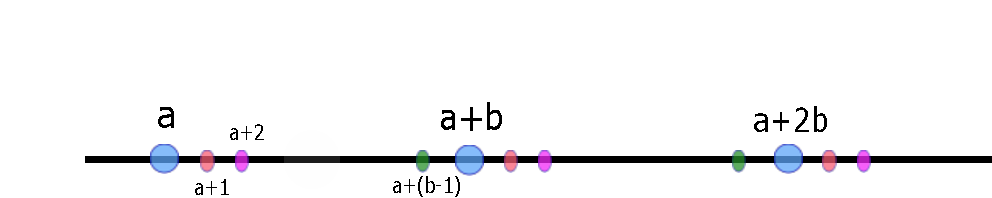
\includegraphics[scale=.4]{fechado.pdf}
\end{center}
\vspace{-7mm}
and $\displaystyle{\bigcup_{i=1}^{b-1}N_{a+i,b}}$ is an open set.  
\end{exampleblock}

\end{frame}

% % ----------------------------------------
\begin{frame}
\frametitle{F\"{u}rstenberg Topological Argument}

\begin{block}{Some properties of closed sets}


  If $X$ is a topological space then:
  \begin{itemize}
    \item[P1.]$\emptyset$ and $X$ are closed sets; 
    \item[P2.] The finite union of closed sets is a closed set;
      \begin{itemize}
      \item  Consider $A_i$, $1 \leq i \leq n$ closed sets. Thus,
        $$X\setminus \displaystyle \bigcup_{i=1}^n A_i = \bigcap_{i=1}^n(X \setminus A_i) \mbox{ is an open set}$$
        \end{itemize}
      \item[P3.] The arbitrary intersection of closed sets is a closed set.
        \begin{itemize}
      \item  Consider $A_{\alpha}$, a family of closed sets. Thus,
        $$X\setminus \displaystyle \bigcap A_{\alpha}= \bigcup(X \setminus A_{\alpha}) \mbox{ is an open set}$$
        \end{itemize}
    \end{itemize}
\end{block}

 \end{frame}  
% % ----------------------------------------

 \begin{frame}
\frametitle{Argumento de F\"{u}rstenberg}

\begin{exampleblock}
  
  \begin{itemize}
  \item \textbf{Statement 4:} Consider $k$ an integer number such that $k \neq 1$ and $k \neq -1$. Therefore, $k$ has a prime divisor $p$ and, consequently, $k \in N_{0,p}$.
   
   Also,
    $$\mathbb{Z} \setminus \{-1,1 \} = \bigcup_{p \in \mathbb{P}} N_{0,p} \mbox{, where } \mathbb{P}
    \mbox{ denotes the set of prime numbers.}$$
  \end{itemize}
  \end{exampleblock}

If $\mathbb{P}$ is finite then:
\begin{itemize}
\item  $\bigcup_{p \in \mathbb{P}} N_{0,p}$ is a closed set (\textbf{Statement 3 + P2});
\item Thus, $\{ -1, 1\}$ is an open set (\textbf{By the definition of a closed set)}.
  \item Consequently $\{ -1, 1\}$ is an infinite set. (\textbf{Statement 1})

  \end{itemize}

  \begin{exampleblock}

    \textbf{Therefore, the set $\mathbb{P}$ of the prime numbers is infinite.}
    \end{exampleblock}
 \end{frame}  



\section*{Refer\^encias}

\begin{frame}[allowframebreaks]
\frametitle{Refer\^{e}ncias}
%----------------------------------------
\footnotesize
%----------------------------------------
\begin{thebibliography}{20}
%\bibliographystyle{apalike}
%----------------------------------------
% \bibitem{avigad14}
% Avigad,J., Harrison, J.: Formally Verified Mathematics.
%   Communication of the ACM
%   \textbf{57}(4) (2014)

% \bibitem{grcr13}
%   Grcr, J.: Errors and Corrections in Mathematics Literature.
%   Notices of AMS. 
%   \textbf{60}(4) (2013)

\bibitem{theBook2018}
  Aigner, Martin and  Ziegler, G\"{u}nter M. Proofs from THE BOOK.
  6th.Springer (2018)


\bibitem{Furstenberg1955}
  Hillel F\"urstenberg. On the Infinitude of Primes.
  Amer. Math, Monthly.
  \textbf{62}(5) (1955)


% \bibitem{Ayala2020}
% M. Ayala-Rincón and T. A. de Lima. Teaching Interactive Proofs to Mathematicians. In Proceedings 9th International Workshop on Theorem Prover Components for Educational Software (ThEdu), 2020.

% \bibitem{MunozN16}
% C{\'{e}}sar A. Mu{\~{n}}oz and
%                Anthony Narkawicz: Formal Analysis of Extended Well-Clear Boundaries for Unmanned Aircraft.
%   NASA Formal Methods - 8th International Symposium, NFM 2016, Minneapolis,
%   MN, USA, June 7-9, 2016, Proceedings.


% \bibitem{AyalaRinconR13}
% Mauricio Ayala{-}Rinc{\'{o}}n and
%                Yuri Santos Rego. Formalization in PVS of Balancing Properties Necessary for Proving
%                Security of the Dolev-Yao Cascade Protocol
%                Model. J. Formalized Reasoning,v6,n.1, pg. 31--61 (2013)
% %---------------------------------------- 
% \bibitem{MunozN13}
% C{\'{e}}sar A. Mu{\~{n}}oz and
%                Anthony Narkawicz. Formalization of Bernstein Polynomials and Applications to Global
%                Optimization. J. Autom. Reasoning. v, 51, n.2,
%                pg. 151--196 (2013)


               

%  \bibitem{Lima21} T. A. de Lima, A. L. Galdino, A. Borges Avelar, and M. Ayala-Rincón. Formalization of Ring Theory in PVS - Isomorphism Theorems, Principal, Prime and Maximal Ideals,Chinese Remainder Theorem. Online Fist, Journal of Automated Reasoning, 2021.
  
% %----------------------------------------  
% \bibitem{yasel14}
% Su{\'{a}}rez, Y.G., Torres, E., Pereira, O., P{\'{e}}rez, C., Rodr{\'{\i}}guez,
%   R.: Application of the ring theory in the segmentation of digital images.
%   International Journal of Soft Computing, Mathematics and Control
%   \textbf{3}(4) (2014)
% %----------------------------------------
% \bibitem{bini12}
% Bini, G., Flamini, F.: Finite commutative rings and their applications,
%   vol.~680. Springer Science \& Business Media (2012)
% %----------------------------------------
% \bibitem{rudolf94}
% Lidl, R., Niederreiter, H.: Introduction to finite fields and their
% applications. Cambridge University Press, Cambridge (1994)


% %----------------------------------------
% \bibitem{hungerford80}
% Hungerford, T.W.: Algebra, Graduate Texts in Mathematics, vol.~73.
%   Springer-Verlag, New York-Berlin (1980), reprint of the 1974 original
% %----------------------------------------
% \bibitem{artin10}
% Artin, M.: {Algebra}. Pearson, 2 edn. (Aug 2010)
% %----------------------------------------
% \bibitem{dummit03}
% Dummit, D.S., Foote, R.M.: {Abstract Algebra}. Wiley, 3 edn. (Jul 2003)
% %----------------------------------------
% \bibitem{herstein75}
% Herstein, I.N.: Topics in algebra. Xerox College Publishing, Lexington,
%   Mass.-Toronto, Ont., 2 edn. (1975)
% %----------------------------------------
% \bibitem{ballarin} Aransay, J., Ballarin, C., Baillon, M., de Vilhena, P.E., Hohe, S., Kammüller, F., Paulson, L.C.: The Isabelle/HOL Algebra Library. Technical report, Isabelle Library, University of Cambridge Computer Laboratory and Technische Universität München (2019). https://isabelle.in.tum.de/dist/library/HOL/ HOL- Algebra/document.pdf
%----------------------------------------

%---------------------------------------- 
%  \bibitem{MCL07}
%   Marc Daumas and
%                David R. Lester and
%                C{\'{e}}sar A. Mu{\~{n}}oz. Verified Real Number Calculations: A Library for Interval Arithmetic.
%  CoRR.
%   v. 0708.3721
%   (2007)
%  %---------------------------------------- 
% \bibitem[AvelarGMA14]
%    AAndr{\'{e}}ia Borges Avelar and
%                Andr{\'{e}} Luiz Galdino and
%                Fl{\'{a}}vio Leonardo Cavalcanti de Moura and
%                Mauricio Ayala{-}Rinc{\'{o}}n. First-order unification in the PVS proof assistant.
%  Logic Journal of the IGPL,
%   v.22,
%   n.5,
%   pag. 758--789,
%   (2014)
%  %---------------------------------------- 
% \bibitem{PVSalgebra}
% Ricky Butler and David Lester.
% A PVS \emph{Theory} for Abstract Algebra.
% Nasa Langley Research Center (2007)
% Available at: {\small
%   http://shemesh.larc.nasa.gov/fm/ftp/larc/PVS-library/pvslib.html}
% (Accessed in September 27, 2019)
% %---------------------------------------- 
% \bibitem{SilvaLG18}
%  Andr{\'{e}}ia B. Avelar da Silva and
%                Thaynara Arielly de Lima and
%                Andr{\'{e}} Luiz Galdino.
% Formalizing Ring Theory in PVS. 
% Interactive Theorem Proving - 9th International Conference, ITP
%                2018,
%   pag. 40--47
% (2018)
  


\end{thebibliography}
%----------------------------------------
\end{frame}






\end{document}
%==========================================================
%==========================================================
%==========================================================
